\section{Organisation du travail}

Pour ce stage au sein de Code Lutin, très vite après avoir pris connaissance 
de mon environnement de travail et des différentes taches qui m'attendait sur
le projet wikitty publication, on m'a demandé un planning prévisionnel du travail
(Planning sur la page suivante).

Pour ce stage, et le projet WikittyPublication, ce qui à été fait, c'est que 
j'ai découpé les specifications de wikitty publication en "grosse" fonctionnalitées
de manière à ce que "régulièrement" il puisse y avoir des choses concrètres qui 
fonctionnent.

Les étapes étaient toujours les mêmes dans ces "cycles" de développement:
\begin{itemize}
\item discussion avec mon maitre de stage sur les attentes
\item rédaction de spécifications, en détaillant les demandes de sorte à être
le moins ambigue possible, envoit de ses spécifications sur la liste de 
développement, discussion éventuelle sur ces propositions
\item implémentation des spécifications, avec mise à jour des spécifications 
si nécessaire
\item tests
\item documentation du code
\end{itemize}

De plus toutes les trois semaines au cours de réunions de développement, je 
présentait l'avancé de mon travail et faisait démonstration du fonctionnement
de Wikitty Publication et des fonctionnalités que j'avais fait depuis la dernière
réunion.

En parallèle toutes les semaines je faisais un compte rendu par mail sur ce que 
j'avais fais la semaine, ce qui m'avais posé problème et ce que je comptais faire
la semaine suivante. 

L'intégralité du projet Wikitty est basé et construit avec maven, l'intégration
continu est faites par un jenkins, le projet se trouve sur une forge permettant
l'assignation de ticket pour les évolutions et les corrections de bug. 
Un sonar est aussi en place pour les métriques et la vérification des règles
de codage pour le code.

Voici mon planning de travail, il y a des taches qui étaient prévu au départ,
et d'autre qui se sont ajoutées au fur et à mesure. 

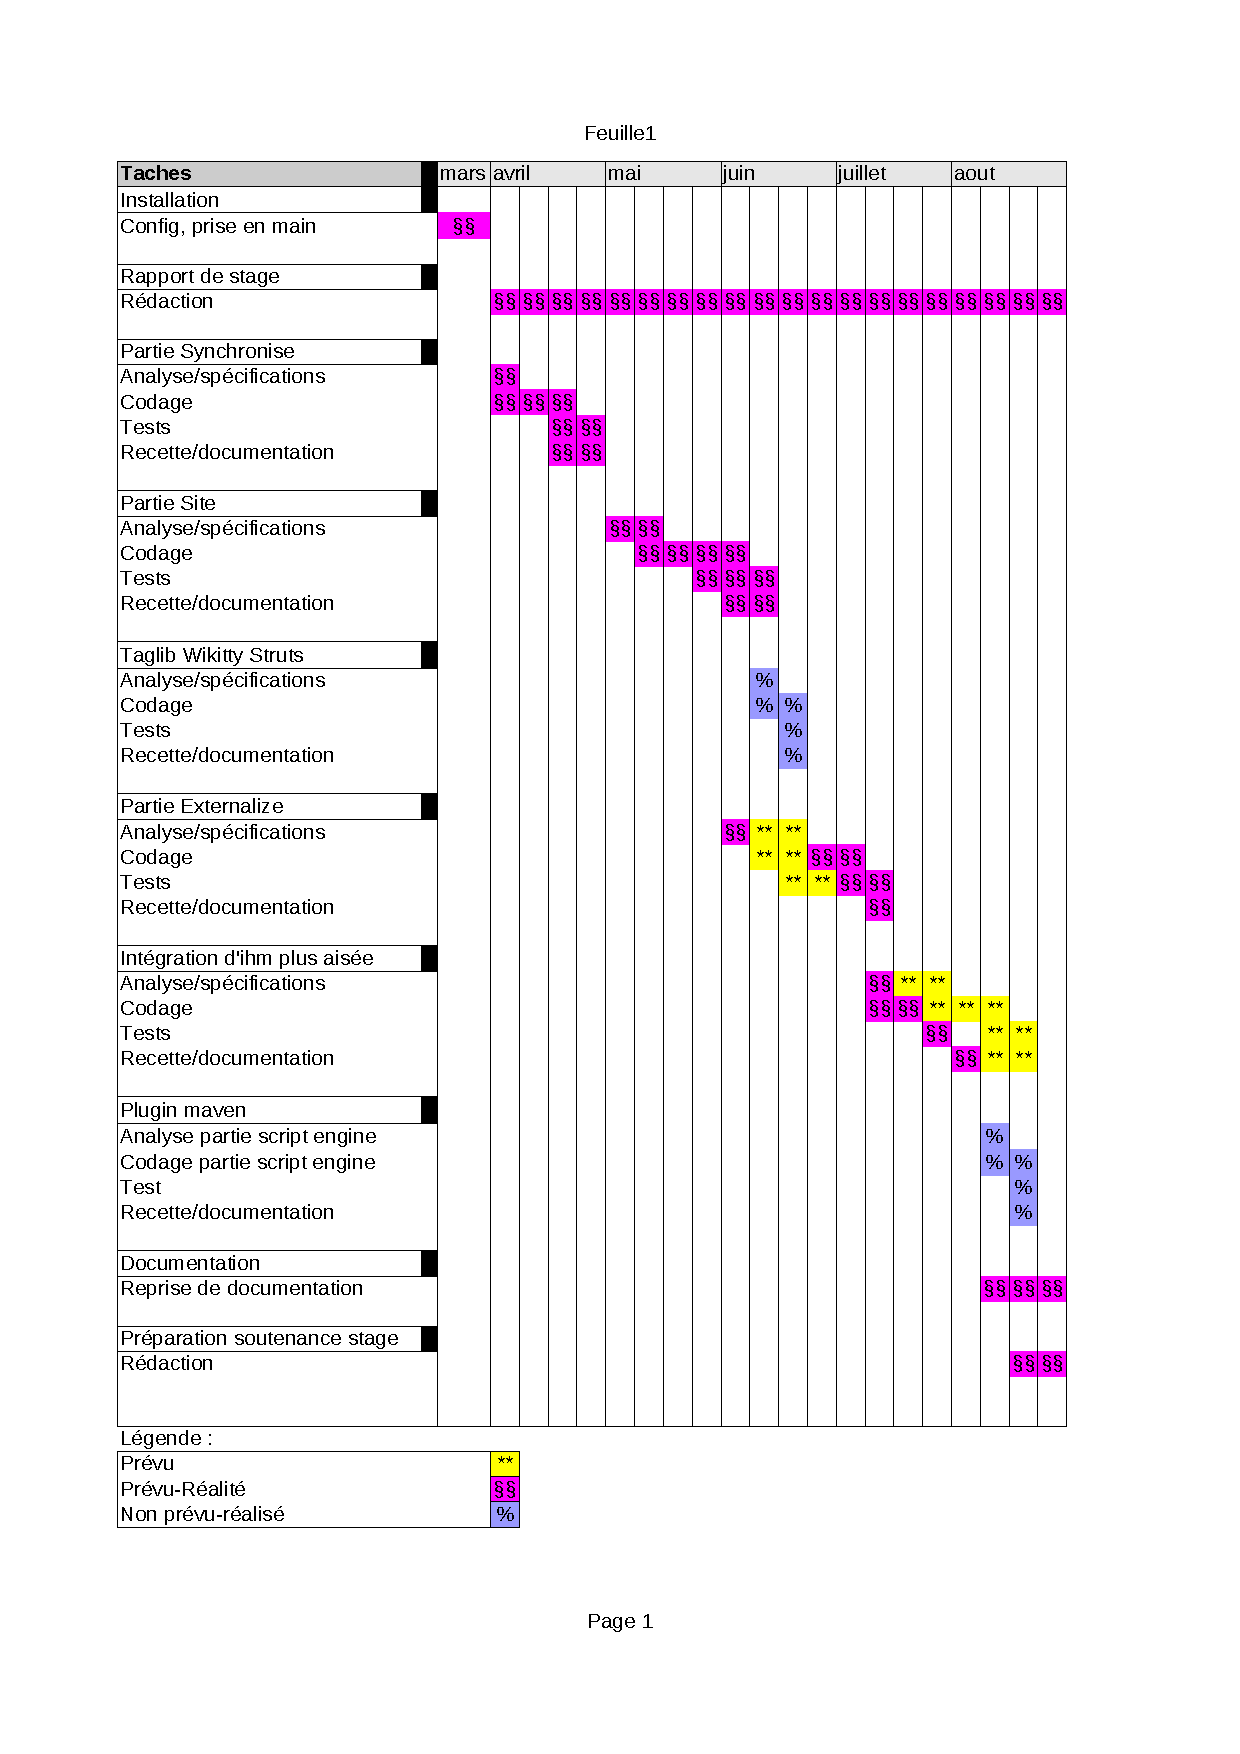
\includepdf{ressources/planningprev2.pdf} 


